\documentclass[a4paper,10pt]{article}
\usepackage[utf8]{inputenc}
\usepackage{graphicx}
\usepackage{float}

\title{Analiza podatkov Food And Drug Administration z orodjem Bokeh}
\author{Neža Belej (63120340), Matej Dolenc (63120178)}


\begin{document}

\maketitle
\pagebreak
\section {Bokeh}

Bokeh je interaktivna knjižnica programskega jezika Python. Omogoča elegantno in interaktivno vizualizacijo nad veliko množico podatkov.
Arhitektura Bokeha sestoji iz dveh delov: izdelava grafov s programskim jezikom Python in pa izris v brskalniku s knjižnico BokehJS. Grafi v Pythonu se pretvorijo v JSON format, saj to zahteva BokehJS. Takšen dizajn je zelo fleksibilen, saj omogoča, da delo tudi z drugimi programskimi jeziki (R, Scala, Lua,... ) lahko privede do enakih Bokeh grafov v brskalniku. 

Če želimo sinhronizacijo Bokeh grafov in interaktivne vizualizacije v brskalniku, moramo uporabiti tudi strežnik Bokeh. Tako imamo omogočeno avtomatično posodabljanje uporabniškega vmesnika v brskalniku glede na naše klike in vnose.

\subsection{Težave}
Med spoznavanjem orodja Bokeh smo opazili, da ima orodje še kar nekaj hroščev. V okviru izdelave smo velikokrat naleteli na repozitorij na Githubu, kjer je trenutno kar 764 odprtih nalog ("issues": https://github.com/bokeh/bokeh/issues). \\Orodje je preprosto za uporabo, ima dobro dokumentacijo, vendar ima še veliko lukenj. 

\vspace{5mm}
Ob prikazu grafa najpogostejših reakcij smo želeli na interaktiven način izvesti prikaz reakcij v različnih časovnih obdobjih.
Zato smo najprej želeli uporabiti element DatePicker, kjer bi lahko izbrali začetni in končni datum. Opazili smo, da ima element v trenutni fazi zelo slab izgled, kar je opisano v sledeči povezavi (issue: https://github.com/bokeh/bokeh/issues/4503). Zato smo poizkusili z uporabo elementa DateRangeSlider, ki naj bi imel na različnih straneh drsnika začetni in končni datum. Element se ni prikazal. To je opisano v povezavi (issue: https://github.com/bokeh/bokeh/issues/2268 ). Zato smo bili primorani uporabiti dva navadna drsnika, enega za začetno, drugo za končno leto. 

\section{Pyton}
Programska koda je spisana v jeziku Python. Uporabljen je bil za poizvedovanje, obdelavo podatkov in na koncu še za gradnjo grafov, na katerih so predstavljeni podatki, ki so bili pridobljeni s poizvedbami.

Vsa programska koda se nahaja v priloženih \textit{.py} datotekah in sicer:
\begin{itemize}
\item{\textit{fda.py} - ta datoteka je namenjena pisanju poizvedb. V njej se nahajo vse poizvedbe, ki so bile uporabljene v tej seminarski nalogi.}
\item{\textit{main.py} - v tej datoteki se nahajajo funkcije, ki prejmejo podatke pridobljene iz predhodno opravljeni poizvedb. Ko so podatki obdelani gredo v izris.}
\item{\textit{plotters.py} - v tej datoteki smo definirali funkcije, ki nam omogočajo izris grafov, kot so vidni na rezultatih analize podatkov. To vključuje lomljenke, histograme in kombinacijske grafe.}

\end{itemize}

\section{OpenFDA}
OpenFDA je projekt, ki ga je ustanovil Taha Kass-Hout z namenom ozaveščanja prebivalstva, odprte dostopnosti do podatkov in, potencialno, reševanja življenj.

OpenFDA (Food and Drug Administration) nam na svojih straneh omogoča dostop do 100 GB velike množice podatkov, kjer lahko poizvedujemo o medicinskih poročilih o zdravilih in hrani; na primer stranski učinki zdravil ali odpoklic prehrambenih produktov. OpenFDA je namenjena predvsem za poizvedbe preko njihovega zmogljivega API-ja, ki ima v ozadju implementiran učinkovit Elastic Search. Ta nam omogoča hitro in preprosto poizvedovanje po podatkih. \\
Podatki, namenjeni prenosu, so razbiti na veliko število datotek v JSON formatu. Če želimo prenesti podatke, moramo paziti, da ob vsaki posodobitvi podatkov znova prenesemo celotno zbirko podatkov. Podatki so v dokumentni, nenormalizirani obliki, kar omogoča hitro iskanje.

\section{Navodila za izvajanje}
Za zagon projekta je potrebno imeti nameščeno orodje Anaconda. Nato iz konzole Bash ali pa Windows-ovega CMD-ja zaženemo ukaz:  \begin{itemize}
\item{\textit{conda install bokeh} }
\end{itemize}

Nato se premaknemo v direktorij, ki vsebuje main.py našega projekta in natipkamo ukaz: 
\begin{itemize}
\item{\textit{bokeh serve .} }
\end{itemize} 
V brskalniku se pomaknemo na \textit{localhost:5006}. 5006 tukaj predstavlja številko vrat (port), ki se nam ob zagonu strežnika izpiše v konzoli. 

\section{Analiza podatkov}
Analizo podatkov sva izvedla na dveh različnih bazah in sicer na bazi Food in na bazi Drugs. Baza Food vsebuje podatke o hrani, prehrambenih dopolnilih in presenetiljivo tudi o kozmetiki. Razloga za to žal ne poznava. Na drugi strani baza Drugs vsebuje podatke o zdravilih in njihovi uporabi.
 
Pri bazi Food naju je zanimala proizvodnja hrane v ameriških zveznih državah, stranski učinki in njihova frekvenca ter odpoklic hrane iz trga.
Pri bazi Drugs naju je zanimalo še posebej kateri stranski učinki so najbolj pogosti pri ljudeh (pri moških, ženskah in skupaj), kako pogosto se stranski učinki pojavljajo pri kombinaciji dveh različih zdravil.

Pri analizi sva pazila, da sva se držala zahtevanega števila obdelanih vrstic (vsaj 1 milijon). To je tudi razvidno iz grafov. Primer: Na sliki o najpogostejših stranskih učinkih  (Figure \ref{reak}) je vsota vseh poročanj zagotovo večja kot 1 milijon.

Na koncu bi omenila še, da vsi podatki veljajo samo za Združene države Amerike.


\subsection{Število poročil o stranskih učinkih glede na neko kombinacijo zdravil}
Graf (Figure \ref{stPor}) nam ponazarja število poročanih stranskih učinkov glede na kombinacijo dveh zdravil. Siva barva pomeni, da ni bilo poročanj o reakcijah; bolj intenzivna barva pomeni večje število poročanih reakcij. Na spodnji sliki tako vidimo, da se največje število stranskih učinkov pojavi pri zdravilih Methotrexate in Humira ter Methotrexate in Enbrel. Ob premiku na želen kvadratek se nam prikažejo imena zdravil in število poročanj.
Za vizualizacijo grafa smo opravili dvojno poizvedovanje:

\begin{itemize}

\item{Pridobitev 10 najpogostejših zdravil: \\ \\ \texttt{https://api.fda.gov/drug/event.json?}\newline \texttt{search=receivedate:[20040101+TO+20161230]} \newline \texttt{\&count=patient.drug.medicinalproduct.exact\&limit=10}}

\item{Štetje poročanj pri tej kombinaciji zdravil: \\ \\ \texttt{https://api.fda.gov/drug/event.json?} \newline \texttt{search=receivedate:[20040101+TO+20170106]} \newline \texttt{+AND+patient.drug.medicinalproduct:REVLIMID} \newline   \texttt{+AND+patient.drug.medicinalproduct:HUMIRA}}
\end{itemize}

\begin{figure}[H]
  \caption{Število poročil o stranskih učinkih glede na kombinacijo dveh zdravil}
  \centering
    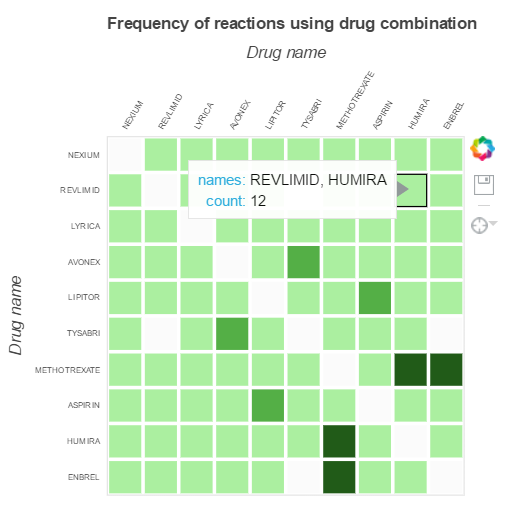
\includegraphics[width=1\textwidth]{kombinacije.png}
    \label{stPor}
\end{figure}

\subsection{Najpogostejši stranski učinki zdravil}
V spodnjem grafu (Figure \ref{reak}) prikazujemo najpogostejše stranske učinke zdravil. Na abscisni osi imamo tako ponazorjeno število poročanj za neko reakcijo. Graf nam omogoča sortiranje glede na spol, čeprav je prikaz obeh spolov ves čas prikazan na grafu. To nam omogoča transparentno pregledovanje podatkov. Filtriranje je možno tudi glede na leto: izberemo lahko začetno in končno leto, torej obdobje, za katero nas zanima število poročanih stranskih učinkov. 

\vspace{5mm}
{\setlength{\parindent}{0cm}
Poizvedba: 
\vspace{5mm}

{\setlength{\parindent}{0cm}
\texttt{https://api.fda.gov/drug/event.json?} \newline \texttt{search=receivedate:[20040101+TO+20170106]+AND+} \newline \texttt{patient.patientsex:2}\& \newline \texttt{count=patient.reaction.reactionmeddrapt.exact} \\
\begin{figure}[H]
  \caption{Najpogostejši stranski učinki}
  \centering
    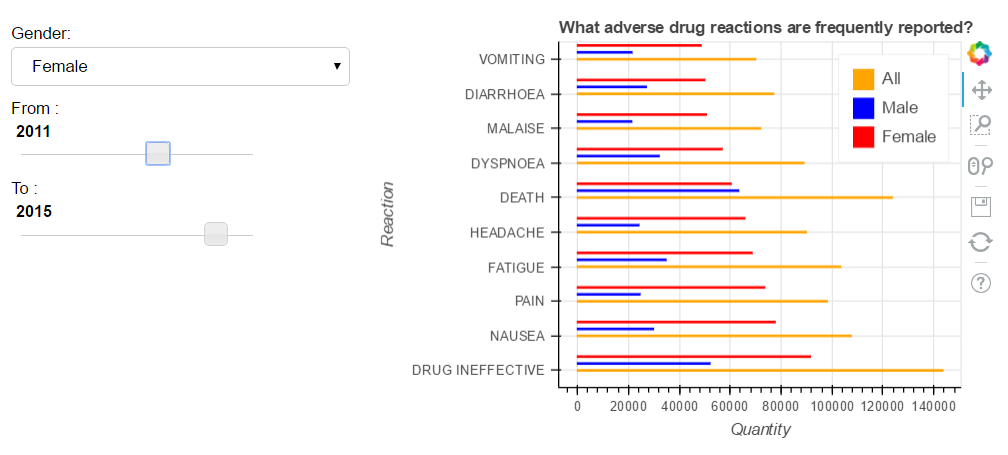
\includegraphics[width=1\textwidth]{reakcije.png}
    \label{reak}
\end{figure}

\subsection{Proizvodnja hrane v ameriških zveznih državah}
Na sledečem grafu (Figure \ref{fP}) je predstavljena proizvodnja hrane v ameriških zveznih državah. S pomočjo tekstovnega polja lahko poljubno izbiramo število mest, ki jih želimo prikazati na grafu. Mesta so urejena od najmanjše proizvodnje do največje proizvodnje. Največ hrane proizvedejo v zvezni državi California (skoraj dvakrat več kot v Teksasu, ki je po proizvodnji hrane na drugem mestu).

\vspace{5mm}
Do teh podatkov pridemo s pomočjo sledeče poizvedbe:

\vspace{5mm}
\texttt{https://api.fda.gov/food/enforcement.json?count=state}



\begin{figure}[H]
  \caption{Proizvodnja hrane v ameriških zveznih državah}
  \centering
    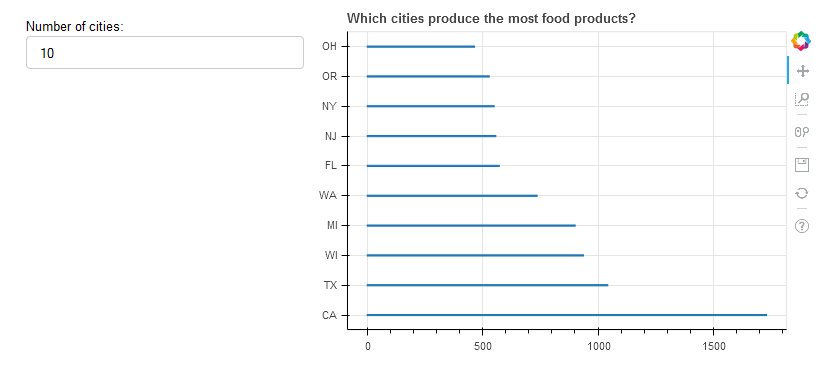
\includegraphics[width=1\textwidth]{foodProd.png}
    \label{fP}
\end{figure}

\subsection{Odpoklic hrane s prodajnih polic po letih}
S pomočjo elementa DatePicker, ki je implementiran v orodju Bokeh, lahko izbiramo tudi datume. To smo uporabili v sledečem primeru, kjer nas je zanimal odpoklic hrane s prodajnih polic po letih. Preden izvedemo poizvedbo, moramo izbrati začetni in končni datum. Kot smo že omenili, je v orodju Bokeh prisotnih kar nekaj hroščev, zato sam izgled elementa DatePicker ni najlepši. Nato poizvedba poišče vse odpoklice, ki padejo v ta datumski interval. Rezultat poizvedbe smo nato obdelali v Pythonu. Končni rezultat je prikazan na grafu (Figure \ref{recall}).

\vspace{5mm}
Do teh podatkov pridemo s pomočjo sledeče poizvedbe:

\vspace{5mm}
\texttt{https://api.fda.gov/food/enforcement.json?}\newline
\texttt{search=recall\_initiation\_date:[20150101+TO+}\newline 
\texttt{20171231]\&count=recall\_initiation\_date}

\begin{figure}[H]
  \caption{Odpoklic hrane s prodajnih polic po letih}
  \centering
    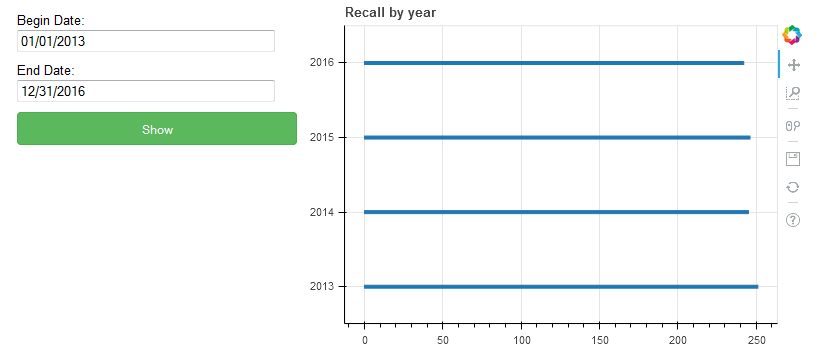
\includegraphics[width=1\textwidth]{recallByYear.png}
    \label{recall}
\end{figure}

\subsection{Stranski učinki hrane, prehranskih dopolnil in kozmetike po letih}
Na sledečem grafu (Figure \ref{ar}) sva želela prikazati število negativnih dogodkov, ki so bili posledica hrane, prehranskih dopolnil ali kozmetike. Za vsako leto je tudi prikazano kakšen je bil skok ali padec glede na prejšnje leto (v procentih). Zanimivo je videti, da so dogodki od leta 2006 do leta 2013 skoraj izključno samo naraščali (izjema je leto 2010). Iz tega bi lahko sklepali, da se v naši hrani, prehrambenih dodatkih in kozmetiki nahaja vedno več umetnih snovi, na katere človek negativno reagira.

\vspace{5mm}
Do teh podatkov pridemo s pomočjo sledeče poizvedbe:

\vspace{5mm}
\texttt{https://api.fda.gov/food/event.json?count=date\_created}
\begin{figure}[H]
  \caption{Stranski učinki hrane, prehranskih dopolnil in kozmetičnih dodatkov po letih}
  \centering
    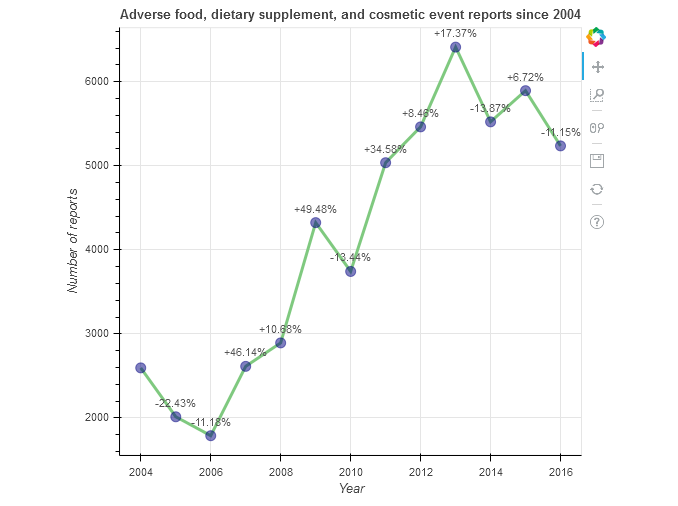
\includegraphics[width=1\textwidth]{adverseReactions.png}
    \label{ar}
\end{figure}


\subsection{Najbolj pogoste skupine hrane, prehranskih dopolnil ali kozmetike, ki povzročajo stranske učinke}

Pri tem grafu (Figure \ref{fpr}) nas je zanimalo katere skupine hrane ali prehranskih dopolnil povzorčajo največ stranskih učinkov. Stranske učinke je mogoče tudi prosto izbirati s pomočjo filtra. Tako lahko pogledamo za specifičen stranski učinek ali pa za vse stranske učinke skupaj. Tukaj sva dobila zelo zanimiv rezultat, saj največ stranskih učinkov povzročajo dodatki kot so vitamini in minerali.

\vspace{5mm}
Primer poizvedbe:

\vspace{5mm}
\texttt{https://api.fda.gov/food/event.json search=outcomes:"serious} \newline
\texttt{+injuries"\&count=products.industry\_name.exact}
   

\begin{figure}[H]
  \caption{Najbolj pogosta hrana ali prehranska dopolnila, ki povzročajo stranske učinke}
  \centering
    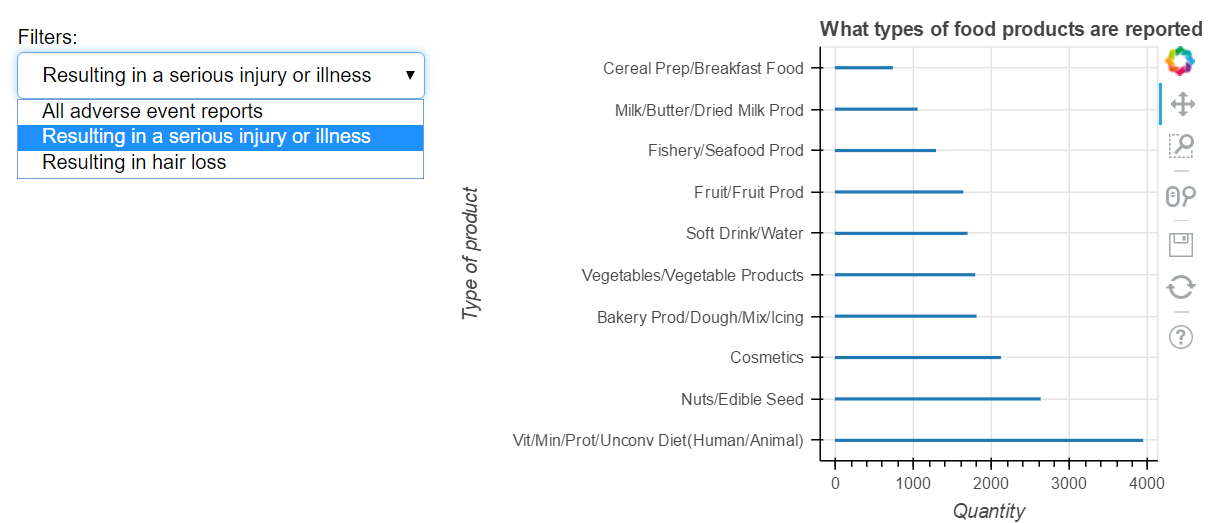
\includegraphics[width=1\textwidth]{tipihrane.png}
    \label{fpr}
\end{figure}

\pagebreak
\section{Reference}
\begin{itemize}
\item {http://bokeh.pydata.org/en/latest/}
\item{https://github.com/bokeh/bokeh/}
\item{https://open.fda.gov/}

\end{itemize}



\end{document}

